\section{The compressible Navier-Stokes equations}

We briefly review the compressible Navier-Stokes equations, given in Section~\secref{sec:compNS}, and formulate DPG for the nonlinear system. 
\begin{itemize}
\item \textbf{Conservation equations}
\begin{align*}
\div \vecttwo{\rho u_1 }{\rho u_2} &= 0\\
\div \vecttwo{\rho u_1^2+p }{\rho u_1 u_2} &= \div\left(\vec{\sigma_{i1}}\right)\\
\div \vecttwo{\rho u_1 u_2}{\rho u_2^2+p } &= \div\left(\vec{\sigma_{i2}}\right)\\
\div\vecttwo{((\rho e)+p)u_1}{((\rho e)+p)u_2} &= \div\left[\boldsymbol\sigma U + \vec{q}\right],
\end{align*}
where $\boldsymbol \sigma$ is the stress tensor whose $ij$th term is $\sigma_{ij}$.  

\item \textbf{Newtonian fluid laws}

We represent $\boldsymbol\sigma$ using the Newtonian fluid law
\[
\sigma_{ij} = \mu(u_{i,j} + u_{j,i}) + \lambda u_{k,k} \delta_{ij}
\]
where $\mu$ is viscosity and $\lambda$ is bulk viscosity. 
%Following elasticity, a general formula for the stress tensor is 
%\[
%\sigma_{ij} = 2\mu \epsilon_{ij} + \lambda \epsilon_{kk} \delta_{ij}
%\]
We can invert the stress tensor under isotropic and plane strain assumptions to get
\[
\frac{1}{2}\left(\grad  U + \grad ^T  U\right) = \frac{1}{2\mu} \sigma_{ij} - \frac{\lambda}{4\mu (\mu + \lambda)} \sigma_{kk}\delta_{ij}
\]
We also have
\[
\frac{1}{2}\left(\grad  U + \grad ^T  U\right) = \grad  U - \boldsymbol \omega
\]
where $\boldsymbol \omega$ is the antisymmetric part of the infinitesimal strain tensor:
\[
\boldsymbol \omega = \frac{1}{2}\left(\grad  U - \grad ^T  U\right).
\]
Thus our final form is
\begin{align*}
\grad  U - \boldsymbol \omega = \frac{1}{2\mu} \boldsymbol \sigma - \frac{\lambda}{4\mu (\mu + \lambda)} { \rm tr}(\boldsymbol \sigma) \boldsymbol I.
\end{align*}
Notice that $\boldsymbol \omega$ is implicitly defined to be the symmetric part of $\grad u$ by taking the symmetric part of the above equation. 

We note that, though this is a standard approach in solid mechanics, it is nonstandard compared to the usual finite element and DG approaches to the viscous stresses. We adopt such an approach to better mirror our experiences with the convection-diffusion equation \cite{DPGrobustness,DPGrobustness2}. 


\item \textbf{Fourier's heat conduction law}

We assume Fourier's law 
\begin{align*}
\vec{q} &= \kappa \grad T,
\end{align*}
%where $\kappa$ is generally a function of temperature. 
We introduce here the Prandtl number here as well
\[
{\rm Pr} = \frac{\gamma c_v \mu}{\kappa}.
\]
In this case, we assume a constant Prandlt number, which implies that the heat conductivity $\kappa$ is proportional to viscosity $\mu$.

\end{itemize}

\subsection{Nondimensionalization}
To nondimensionalize our equations, we introduce nondimensional quantities for length, density, velocity, temperature, and viscosity. 
\[
\boldsymbol x^* = \frac{\boldsymbol x}{L}, \qquad \rho^* = \frac{\rho}{\rho_{\infty}}, \qquad u_1^* = \frac{u_1}{V_\infty}, \qquad u_2^* = \frac{u_2}{V_\infty}, \qquad T^* = \frac{T}{T_\infty}, \qquad \mu^* = \frac{\mu}{\mu_\infty}
\]
Pressure, internal energy, and bulk viscosity are then nondimensionalized with respect to the above variables
\[
p^* = \frac{p}{\rho_\infty V_\infty^2}, \qquad \iota^* = \frac{\iota}{V_\infty^2}, \qquad \lambda^* = \frac{\lambda}{\mu_\infty}
\]
We introduce, for convenience, the Reynolds number
\[
\Reyn = \frac{\rho_\infty V_\infty L}{\mu_\infty} 
\]
and the reference (free stream) Mach number
\[
M_\infty = \frac{V_\infty}{\sqrt{\gamma(\gamma-1)c_vT_\infty}}
\]
Note that 
\[
a = \sqrt{\frac{\gamma p_\infty}{\rho_\infty}} = \sqrt{{\gamma p_\infty}} = \sqrt{\gamma(\gamma-1)c_vT_\infty}
\]
The equations take the same form as before after nondimensionalization, so long as we define new material constants
\[
\tilde{\mu} = \frac{\mu^*}{\Reyn}, \qquad \tilde{\lambda} = \frac{\lambda^*}{\Reyn}, \qquad \tilde{c}_v = \frac{1}{\gamma(\gamma-1)M_\infty^2}, \qquad \tilde{\kappa} = \frac{\gamma\tilde{c}_v\tilde{\mu}}{\rm Pr}
\]
From here on, we drop the $^*$ superscript and assume all variables refer to their nondimensionalized quantities.

To summarize, our system of equations in the classical variables is now
\begin{align*}
\div \vecttwo{\rho u }{\rho v} &= 0\\
\div \left(\vecttwo{\rho u^2+p }{\rho u v} - \boldsymbol \sigma_{1}\right) &=0\\
\div \left(\vecttwo{\rho u v}{\rho v^2+p } - \boldsymbol \sigma_{2}\right) &=0\\
\div \left(\vecttwo{((\rho e)+p)u}{((\rho e)+p)v} - \boldsymbol\sigma \mathbf{u} + \vec{q}\right) &=0\\
\frac{1}{2\mu} \boldsymbol \sigma - \frac{\lambda}{4\mu (\mu + \lambda)} { \rm tr}(\boldsymbol \sigma) \boldsymbol I &= \grad \mathbf{u} - \Reyn \, {\boldsymbol \omega}\\
\frac{1}{\kappa}\vec{q} &= \grad T
\end{align*}
We strongly enforce symmetry of the stress tensor $\boldsymbol \sigma$ by setting $\sigma_{21} = \sigma_{12}$. Additionally, we have scaled the antisymmetric tensor $\boldsymbol \omega$ by the Reynolds number to ensure that $\boldsymbol \omega = O(1)$ for all ranges of $\Reyn$.  

\subsection{Linearization}

\subsubsection{Conservation laws}

The Navier-Stokes conservation laws can be written as 
\begin{align*}
\div \vecttwo{\rho u }{\rho v} &= 0\\
\div \left(\vecttwo{\rho u^2+p }{\rho u v} - \boldsymbol \sigma_{1}\right) &=0\\
\div \left(\vecttwo{\rho u v}{\rho v^2+p } - \boldsymbol \sigma_{2}\right) &=0\\
\div \left(\vecttwo{((\rho e)+p)u}{((\rho e)+p)v} - \boldsymbol \sigma_1 \cdot \boldsymbol u- \boldsymbol \sigma_2 \cdot \boldsymbol u + \vec{q}\right) &=0
\end{align*}
or generally, 
\[
\div (F_i(\boldsymbol U)-G_i(\boldsymbol U,\boldsymbol \sigma) = 0, \qquad i = 1,\ldots, 4
\]
The variational form restricted to a single element gives
\[
\langle \widehat{F}_i\cdot n, v\rangle - \int_K  (F(\boldsymbol U)-G_i(\boldsymbol U,\boldsymbol \sigma)) \cdot \grad v_i = 0 , \qquad i = 1,\ldots, 4
\]
and the variational form over the entire domain is given by summing up the element-wise contributions. 

The presence of terms such as $\boldsymbol \sigma_i \cdot \boldsymbol u$ means that we will need to linearize in the stress variables $\sigma_ij$ in addition to our Eulerian quantities. Since fluxes and traces are linear, we do not need to linearize them. Instead, fluxes $\widehat{F}_{i,n}$ and traces $\widehat{u},\widehat{v},\widehat{T}$ will represent normal traces and traces of the accumulated nonlinear solution. The linearized variational formulation is thus
\begin{align*}
\langle \widehat{F}_i\cdot n, v\rangle &- \int_K  \left(F_{i,\boldsymbol U}(\boldsymbol U)\cdot \Delta \boldsymbol U -G_{i,\boldsymbol U}(\boldsymbol U, \boldsymbol \sigma)\cdot \Delta \boldsymbol U - G_{i,\boldsymbol \sigma}(\boldsymbol U, \boldsymbol \sigma)\cdot \Delta \boldsymbol \sigma \right)\cdot \grad v_i \\
&= \int_K  \left(F_i(\boldsymbol U)-G_i(\boldsymbol U)\right) \cdot \grad v_i \\
\qquad i &= 1,\ldots, 4
\end{align*}
where $F^i_{j,\boldsymbol U}$, $G^i_{j,\boldsymbol U}$, and $G^i_{j,\boldsymbol \sigma}$ are the Eulerian and two viscous Jacobians (linearized w.r.t.\ the Eulerian/viscous variables), respectively.
%where
%\begin{align*}
%F^1_{1,\boldsymbol U} &= \{u,\rho ,0,0\} \\
%F^2_{1,\boldsymbol U} &= \{v,0,\rho ,0\} \\
%F^1_{2,\boldsymbol U} &=\left\{c_v T (\gamma -1)+u^2,2 u \rho ,0,c_v (\gamma -1) \rho \right\}\\
%F^2_{2,\boldsymbol U} &=\{u v,v \rho ,u \rho ,0\}\\
%F^1_{3,\boldsymbol U} &=\{u v,v \rho ,u \rho ,0\}\\
%F^2_{3,\boldsymbol U} &=\left\{c_v T (\gamma -1)+v^2,0,2 v \rho ,c_v (\gamma -1) \rho \right\}\\
%F^1_{4,\boldsymbol U} &=\left\{\frac{1}{2} u \left(2 c_v T (2 \gamma -1)+u^2+v^2\right),\frac{1}{2} \rho  \left(2 c_v T (2 \gamma -1)+3 u^2+v^2\right),u v \rho ,c_v u (2 \gamma -1) \rho \right\}\\
%F^2_{4,\boldsymbol U} &=\left\{\frac{1}{2} v \left(2 c_v T (2 \gamma -1)+u^2+v^2\right),u v \rho ,\frac{1}{2} \rho  \left(2c_v T (2 \gamma -1)+u^2+3 v^2\right),c_v v (2 \gamma -1) \rho \right\}
%\end{align*}
%The viscous Jacobians become (when linearized with respect to $\{\sigma_{11},\sigma_{12}, \sigma_{22}\}$)
%\begin{align*}
%G^1_{2,\boldsymbol \sigma} &= \{1,0,0\}\\
%G^2_{2,\boldsymbol \sigma} &= \{0,1,0\}\\
%G^1_{3,\boldsymbol \sigma} &= \{0,1,0\}\\
%G^2_{3,\boldsymbol \sigma} &= \{0,0,1\}\\
%G^1_{4,\boldsymbol \sigma} &= \{u_1,u_2,0\}\\
%G^2_{4,\boldsymbol \sigma} &= \{0,u_1,u_2\}
%\end{align*}
%and (when linearized with respect to the Eulerian variables)
%\begin{align*}
%G^1_{4,\boldsymbol U} &= \{0,\sigma_{11},\sigma_{12},0\}\\
%G^2_{4,\boldsymbol U} &= \{0,\sigma_{12},\sigma_{22},0\}
%\end{align*}

\subsubsection{Viscous equations}
We have two equations left to linearize - the constitutive laws defining our viscous stresses and heat flux terms. 
\begin{align*}
\frac{1}{2\mu}{\boldsymbol \sigma}- \frac{\lambda}{4\mu(\mu+\lambda)}{\rm tr}({\boldsymbol \sigma}){\boldsymbol I} + \Reyn {\boldsymbol \omega} &= 
\grad
\left[\begin{array}{c}
u_1\\
u_2
\end{array}
\right]\\
\frac{1}{\kappa}
\left[\begin{array}{c}
q_1\\
q_2
\end{array}\right] &=
\grad T
\end{align*}

We treat the first tensor equation as two vector equations by considering each column:
\begin{align*}
\frac{1}{2\mu} \vecttwo{\sigma_{11}}{\sigma_{12}} - \frac{\lambda}{4\mu(\mu+\lambda)}\vecttwo{\sigma_{11}+\sigma_{22}}{0} + \Reyn\vecttwo{0}{-\omega} - \grad u_1&= 0 \\
\frac{1}{2\mu} \vecttwo{\sigma_{12}}{\sigma_{22}} - \frac{\lambda}{4\mu(\mu+\lambda)}\vecttwo{0}{\sigma_{11}+\sigma_{22}} + \Reyn\vecttwo{\omega}{0} - \grad u_2 &= 0
\end{align*}
%These equations are linear in $\sigma_{ij}$, so the linearization is simple. 
Since all equations are linear in variables $q_1, q_2, w$ for all combinations of variables, we do not need to linearize any equations in $q_1, q_2, w$. 

We do not linearize the viscosities $\mu$ and $\lambda$, but instead set them based on the power law and the solution at the previous timestep for simplicity. 

\subsection{Test norm}

Recall the convection-diffusion problem 
\begin{align*}
\div \left(\beta u - \sigma\right) &= f\\
\frac{1}{\epsilon}\sigma - \grad u &= 0.
\end{align*}
On domain $\Omega$, with mesh $\Oh$ and mesh skeleton $\Gh$, the DPG variational formulation is
\begin{align*}
b\left(\left(u,\sigma, \widehat{u}, \widehat{f}_n\right),
\left( v, \tau \right)\right) = \left(u,\div \tau - \beta \cdot \grad
v\right)_{\Oh} + \left(\sigma, \epsilon^{-1} \tau + \grad v\right)_{\Oh} - \LRa{
\jump{\tau\cdot n}, \widehat{u} }_{\Gh} + \LRa{ \widehat{f}_n,
  \jump{v} }_{\Gh}.
\end{align*}
with $v\in H^1$ and $\tau \in H({\rm div},\Oh)$. The test norm adopted for convection-diffusion in Section~\secref{sec:testNormSec} and in \cite{DPGrobustness2} is defined elementwise on $K$ as
\[
\|\left(v,\tau\right)\|_{V,K}^2 = \min\left\{\frac{\epsilon}{|K|},1\right\}\|v\|^2 + \epsilon \|\grad v\|^2 + \|\beta \cdot \grad v\|^2 + \| \div \tau\|^2 + \min\left\{\frac{1}{\epsilon},\frac{1}{|K|}\right\}\|\tau\|^2.
\]
This test norm both delivers robust control of the error in the $L^2$ variables $u$ and $\sigma$ and avoids boundary layers in the computation of local test functions. 

Our test norm is extrapolated to the Navier-Stokes equations as follows: we denote the vector of $H^1$ test functions as $v=\{v_1,v_2,v_3,v_4\}$, and similarly for $W = \{\tau_1,\tau_2,\tau_3\}$. Similarly, we group our Eulerian and stress variables into the vector variables $U$ and $\Sigma$, respectively. If $R_{\rm Euler}(U,\Sigma)$ and $R_{\rm visc}(U,\Sigma)$ are Eulerian and viscous nonlinear residuals, our formulation for the linearized Navier-Stokes equations can be written as
\begin{align*}
\div \left(A_{\rm Euler}U - A_{\rm visc}\Sigma\right) &= R_{\rm Euler}(U,\Sigma)\\
E_{\rm visc} \Sigma - \grad U &= R_{\rm visc}(U,\Sigma)
\end{align*}
with variational formulation
\begin{align*}
\LRa{\widehat{F}_n,V}_{\Gh} + \left(U,\div W - A_{\rm Euler}^T\grad  V\right) + \LRa{\widehat{U},W\cdot n}_{\Gh} + \left(\Sigma,E_{\rm visc}^TW - A_{\rm visc}^T\grad  V\right) &= 0
\end{align*}
Identifying vector-valued terms in the Navier-Stokes formulation with equivalent scalar terms in the convection-diffusion equation allows us to extrapolate our test norm to systems of equations
\begin{align*}
\|\left(V,W\right)\|_{V,K}^2 =& \min\left\{\frac{\Reyn}{|K|},1\right\}\|v\|^2 + \frac{1}{\Reyn} \|A_{\rm visc}^T\grad v\|^2 + \|A_{\rm Euler}^T \grad v\|^2 \\
& + \| \div W\|^2 + \min\left\{\Reyn,\frac{1}{|K|}\right\}\|E_{\rm visc}^T\tau\|^2.
\end{align*}
An advantage of this extrapolation approach is that the incompletely parabolic nature of the Navier-Stokes equation is taken into account; there is no diffusive term present in the mass conservation equation, and the test norm reflects that by requesting only limited regularity of $v_1$.\footnote{The situation is analagous to using the full $H^1(\Oh)$ norm for the pure convection equation --- the optimal test norm $\nor{v}_V = \nor{\beta\cdot \grad v} + \nor{v}$ implies only streamline regularity, whereas taking $\nor{v}_V = \nor{\grad v} + \nor{v}$ implies stronger regularity on the test space $V$ than the graph norm. Consequently, convergence is suboptimal for DPG applied to the convection problem under the $H^1(\Oh)$ test norm.}

\subsection{Boundary conditions}

As a consequence of the ultra-weak variational formulation, our solution is linear in the flux and trace variables. Thus, the nonlinear boundary conditions can be applied directly to our fluxes $\widehat{f}_{i,n}, i = 1,\ldots,4$, and traces $\widehat{u}_1$, $\widehat{u}_2$, and $\widehat{T}$. 

Additionally, inflow boundary conditions are applied not directly to the trace variables $\widehat{u}_1$, $\widehat{u}_2$, and $\widehat{T}$, but to the fluxes $\widehat{f}_{i,n}$. Extrapolating from the convection-diffusion problem, this allows us to use a stronger test norm without experiencing adverse effects for smaller diffusion/higher Reynolds numbers \cite{DPGrobustness,DPGrobustness2}.

\subsection{Numerical experiments: Carter flat plate}

For our solver, we use a standard pseudo-time solver and greedy refinement scheme. Though we have not yet implemented adaptive timestepping, we are able to take large enough uniform timesteps over a coarse mesh such that convergence is order-of-magnitude comparable to the convergence of a damped Newton method. 

The numerical parameters used are as follows:
\begin{itemize}
\item{DPG parameters:} $p = 2$ or $p=3$, and $\Delta p = 2$ uniformly across the mesh. 
\item{Adaptivity parameters:} Energy threshold for refinements is $\alpha = .2$ or $\alpha = .15$. 
\item{Time-stepping parameters:} $\Delta t = .1$, and tolerance for transient residual $\epsilon_t = 5e-7$.
\end{itemize}

Our problem of interest is the Carter flat plate problem. An infinitesmally thin flat plate disrupts a free stream flow and causes a shock to form at the tip of the plate. 

\begin{figure}[!h]
\centering
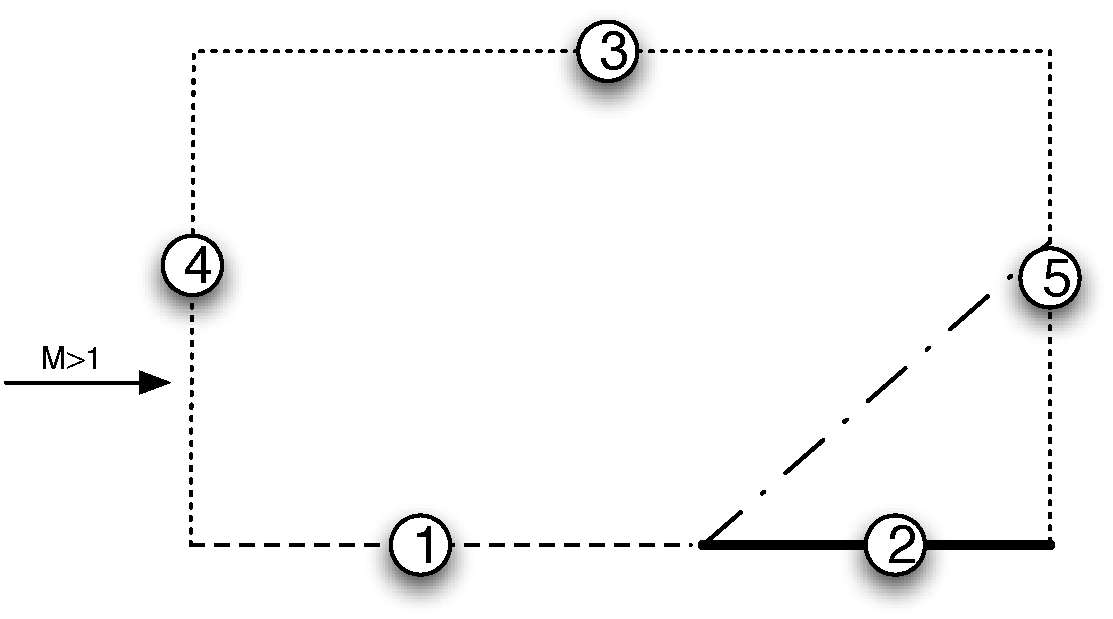
\includegraphics[scale=.5]{figs/flat_plate_BCs.pdf}
\caption{Carter flat plate problem.}
\end{figure}

\begin{itemize}
\item \textbf{Inflow boundary conditions:} free stream conditions are applied here to all four fluxes $\widehat{f}_{i,n}$.
\item \textbf{Symmetry boundary conditions:} $u_n = q_n = \pd{u_s}{n} = 0$. Here, this implies $u_2 = q_2 = \sigma_{12} = 0$. We impose the stress condition by noting that, for the flat plate geometry, if $u_2 = 0$, then at the top and bottom, with $n = (0,1)$, $\widehat{f}_{2,n} = \sigma_{12}$, and $\widehat{f}_{4,n} = q_2$ if $\sigma_{12}$ and $u_2 = 0$. 
\item \textbf{Flat plate boundary conditions:} $u_1 = u_2 = 0$, and $T = T_w = \left[1+(\gamma-1)M_\infty^2/2\right] T_\infty = 2.8T_\infty$ (for Mach 3 flow). We impose these strongly on the trace variables $\widehat{u}_1, \widehat{u}_2, \widehat{T}$. 
\item \textbf{Outflow boundary conditions:} the exact boundary conditions to enforce here are not universally agreed on\footnote{Demkowicz et al enforce an outflow boundary condition only in regions where the flow is subsonic.\cite{Demkowicz:1990:NFE:112271.112276}}. Many enforce $\pd{u_1}{n}=\pd{u_2}{n}=0$ and $\pd{T}{n} = 0$. We adopt a ``no boundary condition'' outflow condition, first introduced in \cite{FLD:FLD1650140506}. A mathematical analysis and explanation of this boundary condition for standard $H^1$ elements is given in \cite{FLD:FLD505}. 

An alternative boundary condition would be as follows: since $u_1$ and $u_2$ are not expected to be zero at these points, we can set $\widehat{f}_{2,n}$ and $\widehat{f}_{4,n}$ to their represented quantities using either the field variables from the background flow, or (in the case of pseudo-time stepping) the previous timestep's flux and field quantities. 

\end{itemize}

We initialize our solution to
\[
\rho = 1,\qquad u_1= 1,\qquad u_2 = 0, \qquad T = 1
\]
which is consistent with what was done in Demkowicz and Oden in \cite{Demkowicz:1990:NFE:112271.112276}. Stresses are set uniformly to zero. 

We take the computational domain to be $\Omega = [0,2]\times[0,1]$. For $\Reyn = 1000$, we experimented with initial meshes from size 4 by 8 to 8 by 16 elements. We note that, on a very coarse initial mesh (4 by 8 elements), the convergence of the pseudo-timestep stagnates at around a transient residual of $1e-6$; however, if we lower the tolerance only for the first step and continued with the adaptive algorithm, the solution converges below $\epsilon_t$ for all refined meshes. 

\begin{figure}[!h]
\centering
\subfigure[$\rho$]{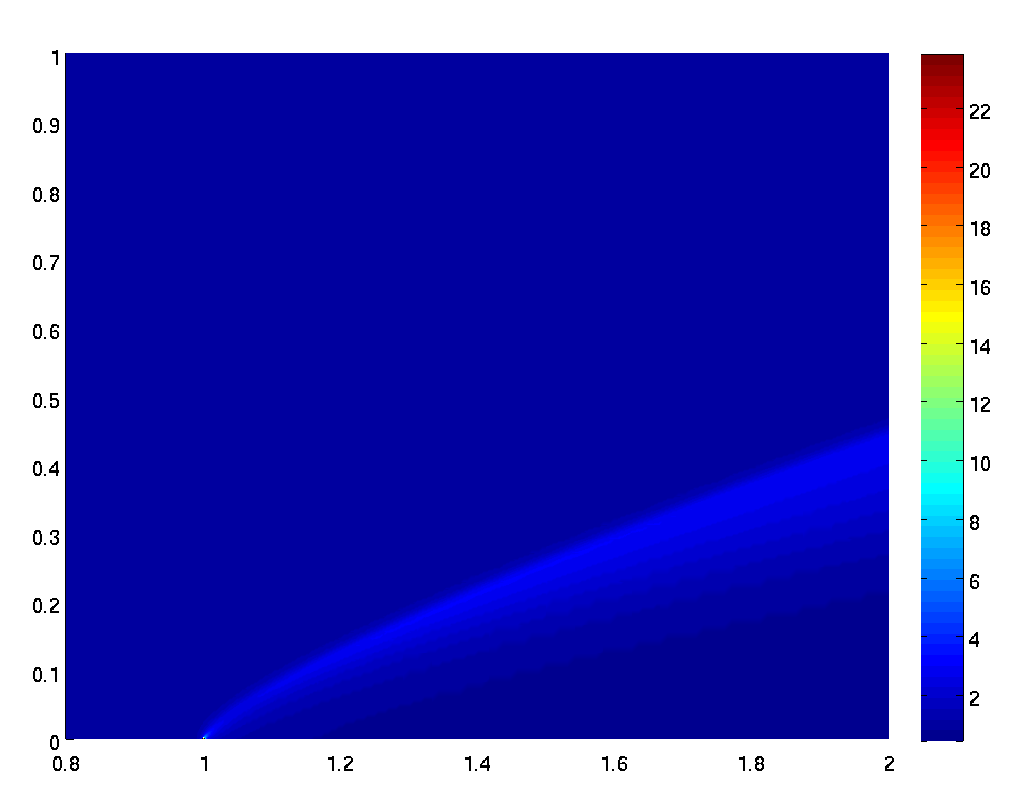
\includegraphics[scale=.42]{figs/Re1000p2/rho.pdf}}
\subfigure[$u_1$]{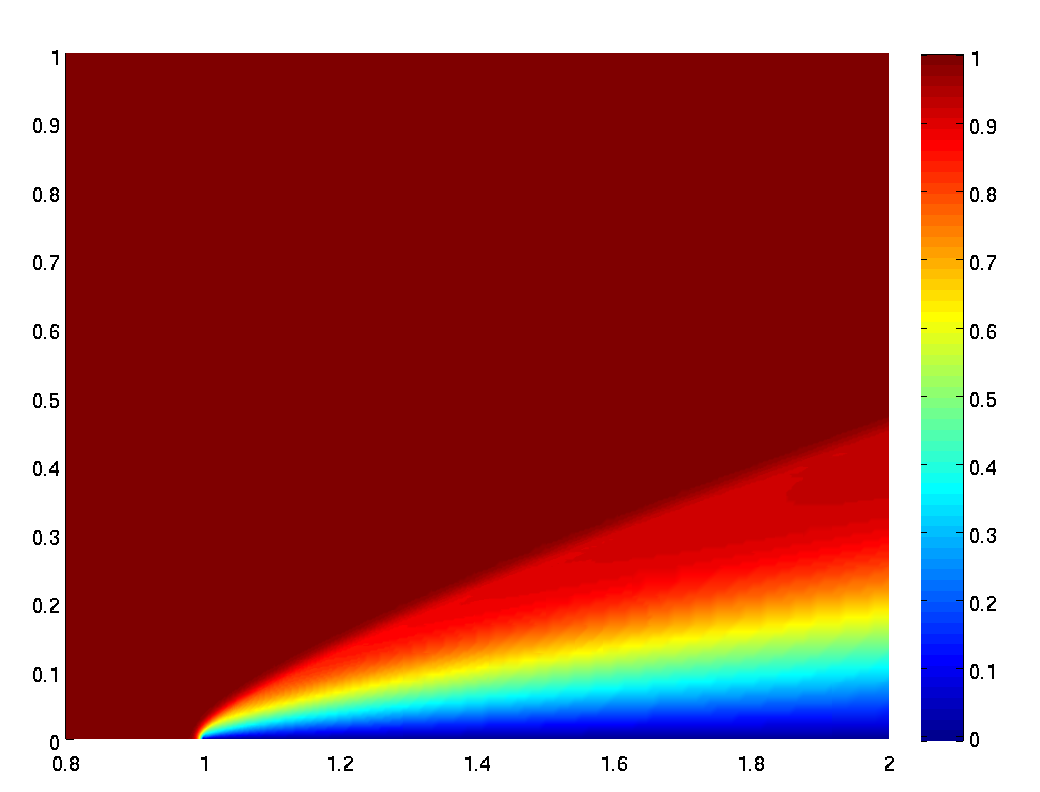
\includegraphics[scale=.42]{figs/Re1000p2/u1.pdf}}
\subfigure[$u_2$]{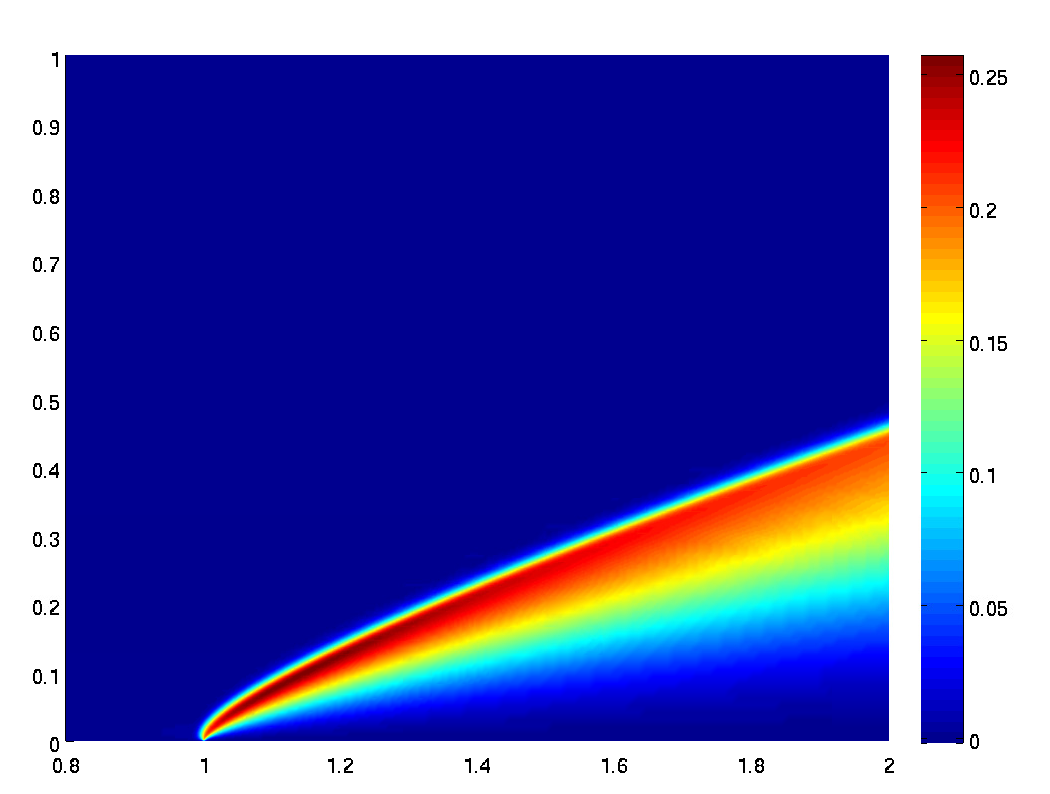
\includegraphics[scale=.42]{figs/Re1000p2/u2.pdf}}
\subfigure[$T$]{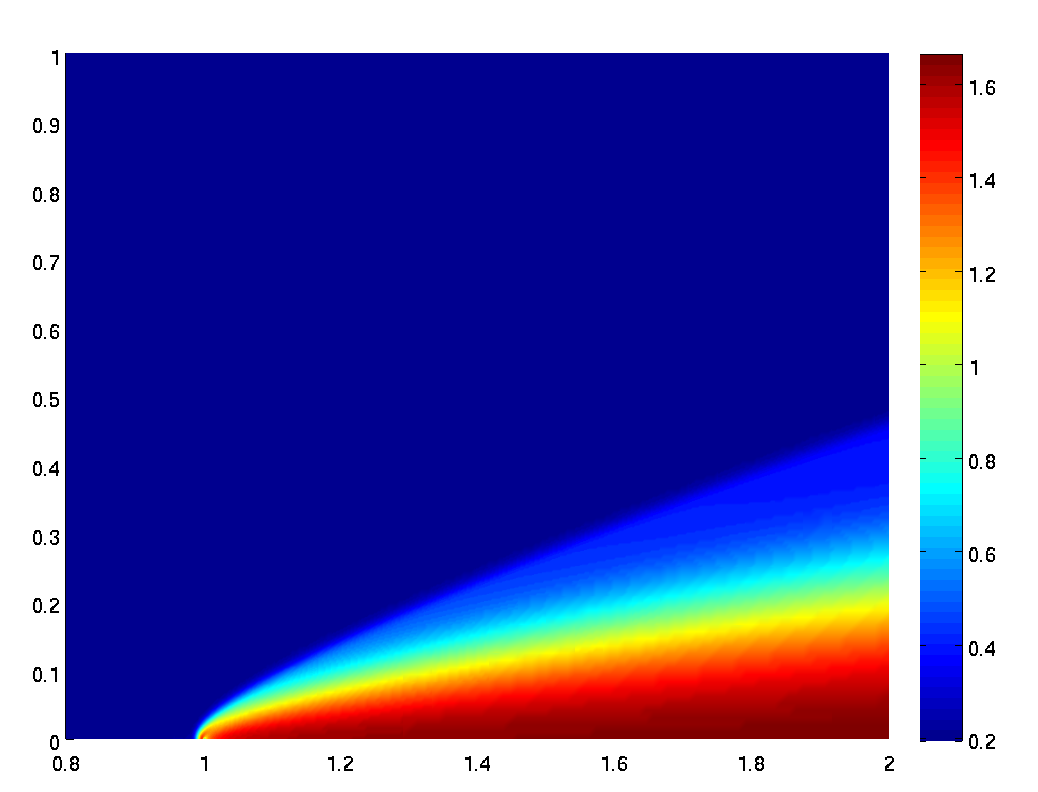
\includegraphics[scale=.42]{figs/Re1000p2/T.pdf}}
\caption{Solutions after six refinements for $p=2$ and $\Reyn = 1000$.}
\label{fig:Re500}
\end{figure}

\begin{figure}[!h]
\centering
\subfigure[$\rho$]{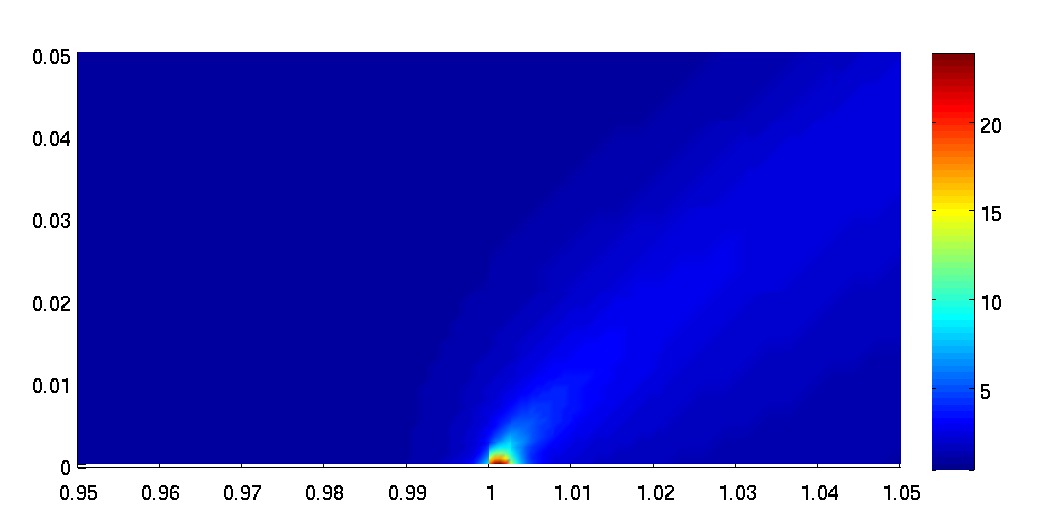
\includegraphics[scale=.4]{figs/Re1000p2/rhozoom.pdf}}
\subfigure[$u_1$]{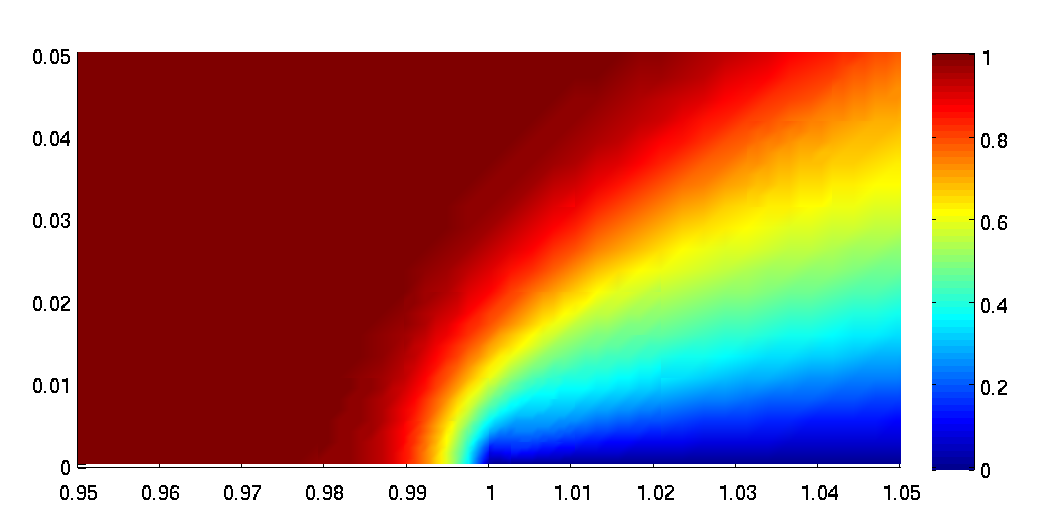
\includegraphics[scale=.4]{figs/Re1000p2/u1zoom.pdf}}
\subfigure[$u_2$]{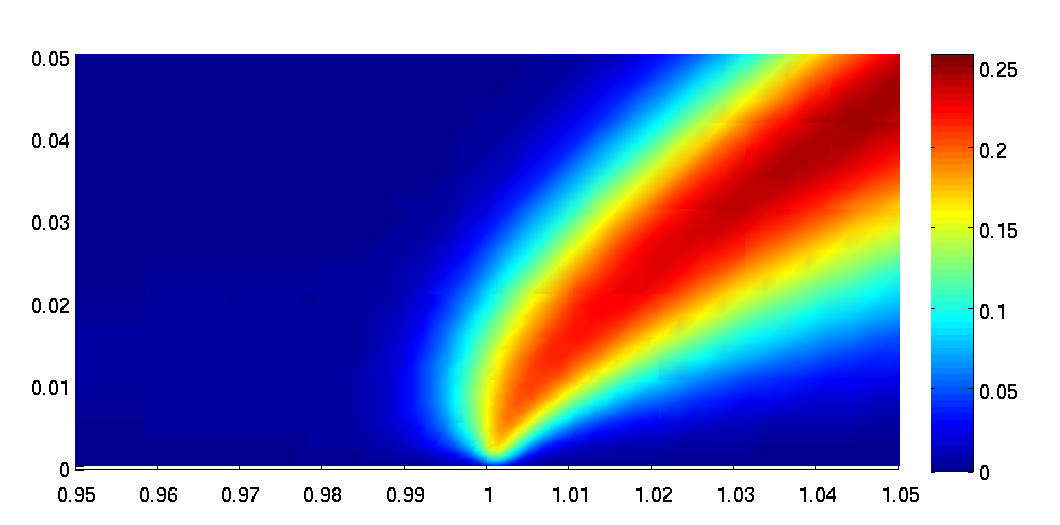
\includegraphics[scale=.4]{figs/Re1000p2/u2zoom.pdf}}
\subfigure[$T$]{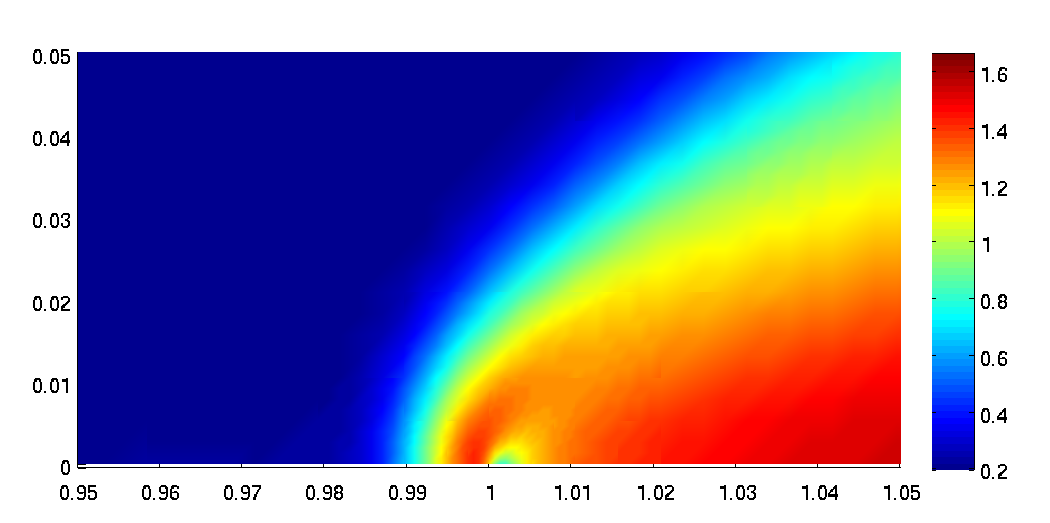
\includegraphics[scale=.4]{figs/Re1000p2/Tzoom.pdf}}
\caption{Zoom of solutions at the beginning of the plate for $p=2$ and $\Reyn = 1000$.}
\label{fig:Re500}
\end{figure}

%For $p=2$, after six refinements, the energy error is 0.000410347. After refinement, mesh has 1083 elements and 143910 global dofs. 

\begin{figure}[!h]
\centering
%\subfigure[$p=2$]{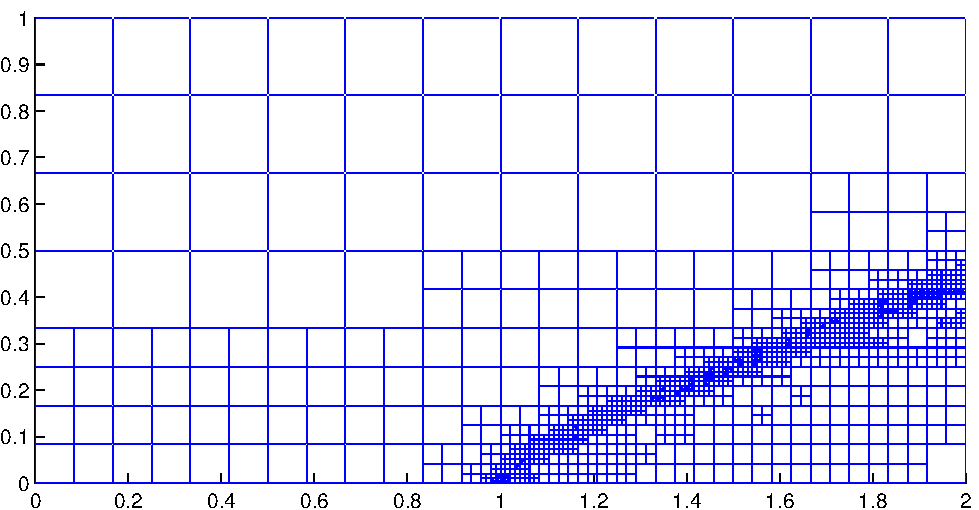
\includegraphics[scale=.5]{figs/Re1000p2/mesh.pdf}}
%\subfigure[$p=3$]{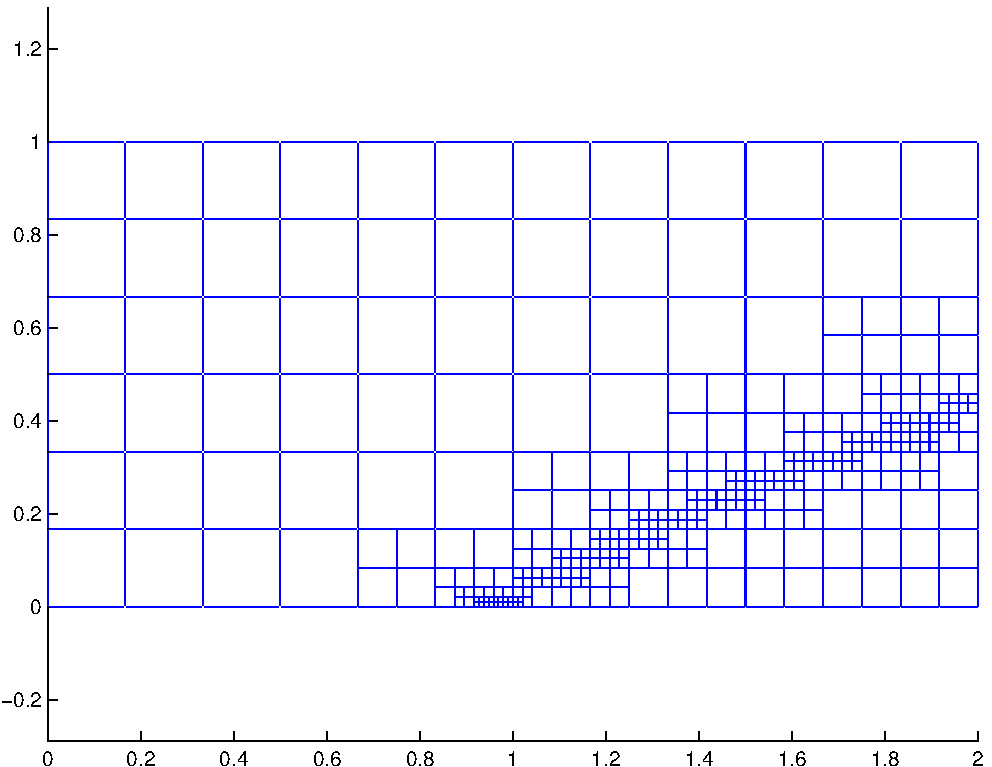
\includegraphics[scale=.5]{figs/Re1000p3/mesh.pdf}}
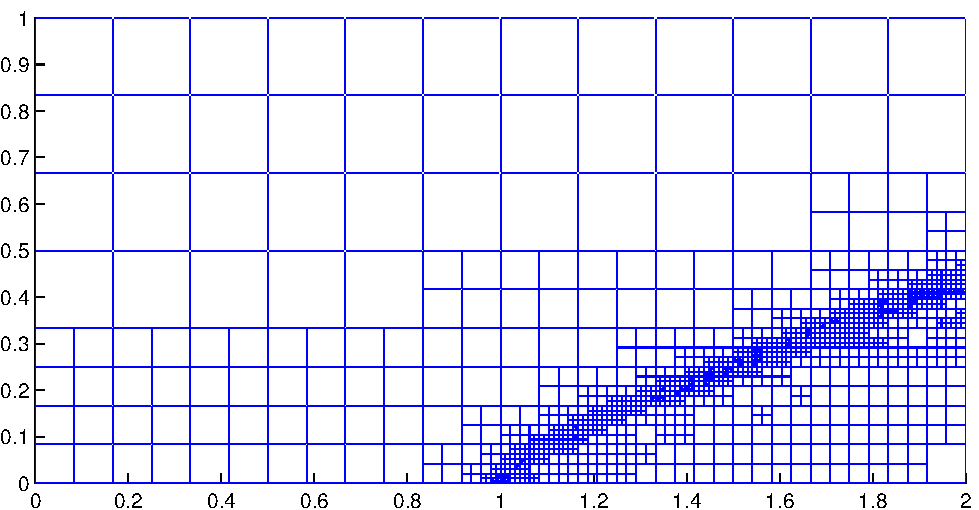
\includegraphics[scale=.55]{figs/Re1000p2/mesh.pdf}
\caption{Adaptive mesh after six refinements for $p=2$
% and five refinements for $p=3$ 
with $\Reyn = 1000$.}
\label{fig:MeshRe1000}
\end{figure}
